%versi 2 (8-10-2016)
\chapter{Landasan Teori}
\label{chap:teori}

\section{KIRI Website }
\label{sec:KIRI} 
KIRI adalah aplikasi navigasi angkutan umum berbasis web yang melayani Bandung dan kota-kota lain di Indonesia.\cite{pascal:17:KIRI}.
Pada awal pembuatannya KIRI dibuat untuk tujuan komersial. Namun karena dinilai kurang sukses project KIRI sekarang menjadi open source project yang dapat di akses. Aplikasi KIRI memiliki beberapa fitur sebagai berikut:
\begin{itemize}
    \item Pemilihan rute tercepat menggunakan angkutan kota.
    \item Menampilkan tempat pergantian angkutan kota.
    \item Memiliki fitur multi bahasa.
    \item Memiliki fitur pemilihan lokasi.
    \item Dapat menampilkan beberapa pilihan rute.
    \item Dapat menampilkan instruksi lengkap  mencapai tujuan.
\end{itemize}

\begin{figure}[H]
    \centering
    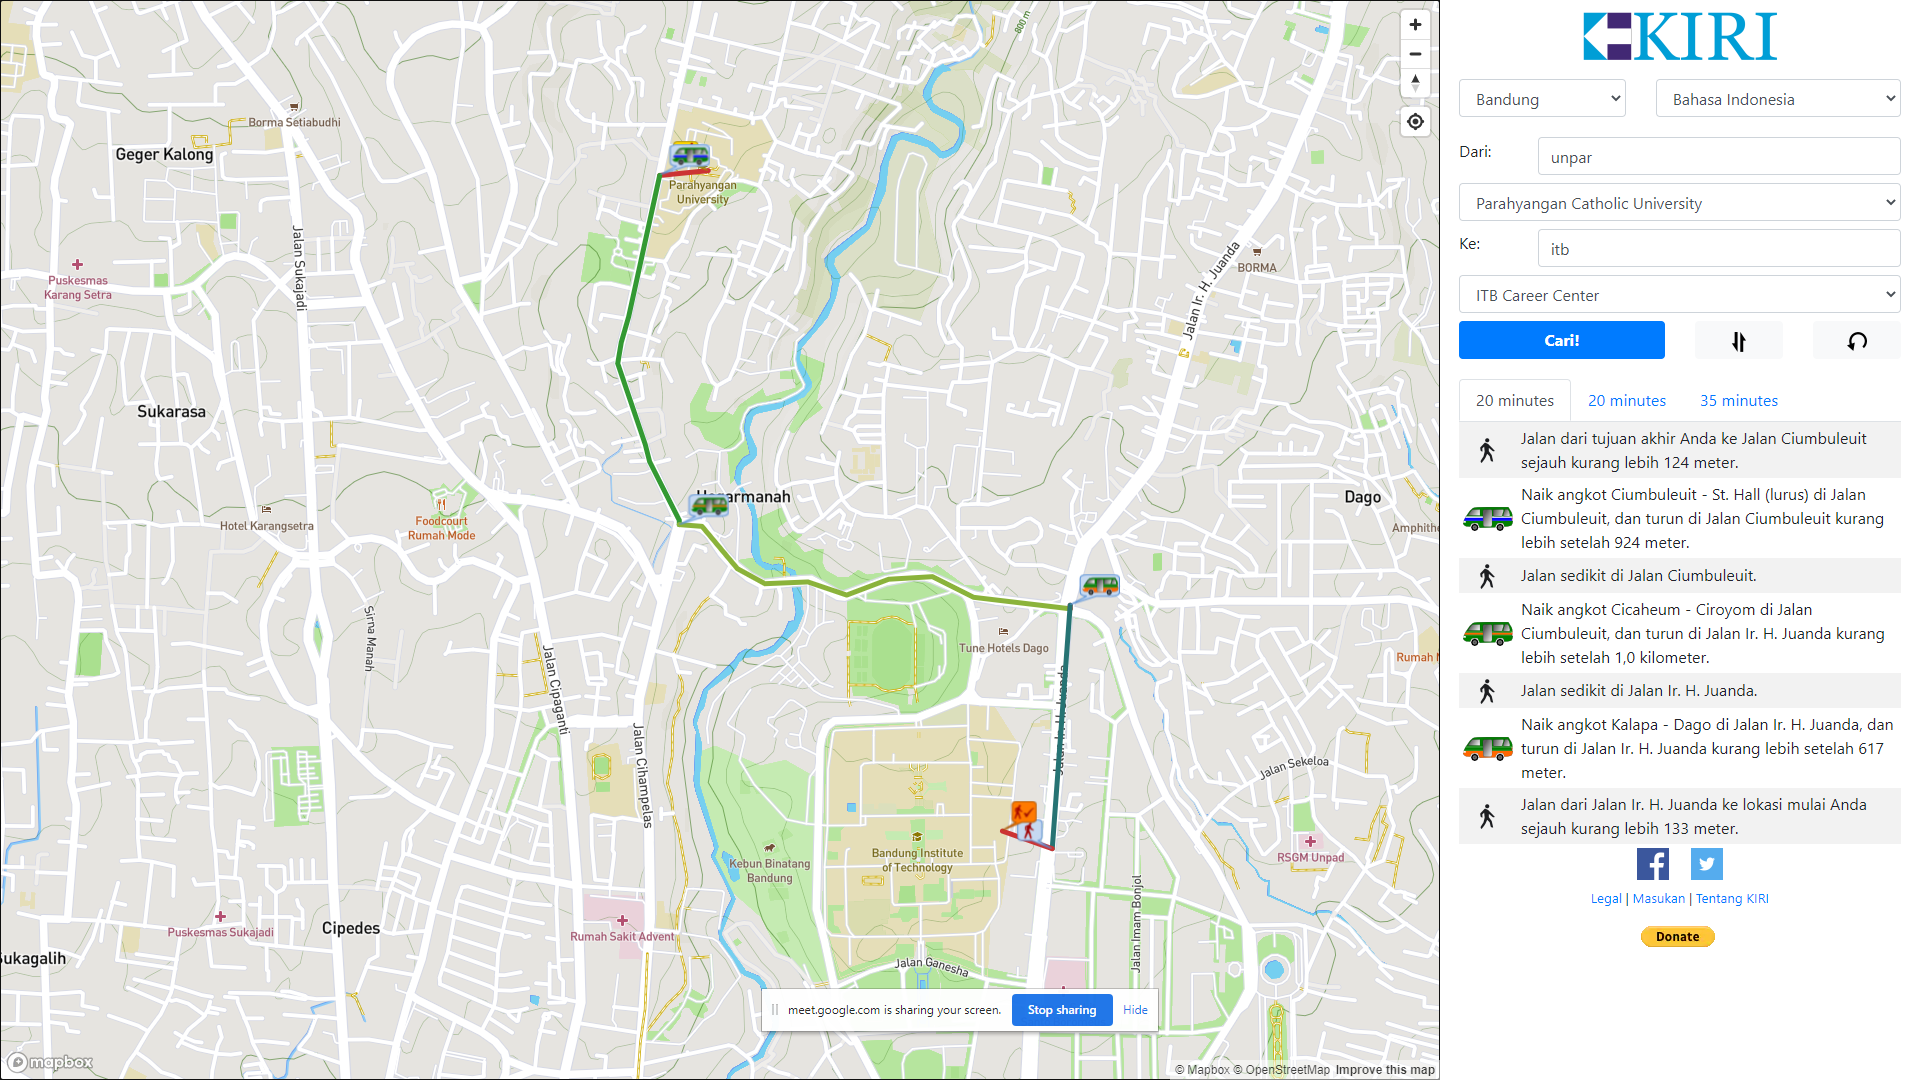
\includegraphics[scale=0.3]{Gambar/kiri-example-1}
    \caption{Tampilan utama website KIRI}
    \label{fig:my_label}
\end{figure}




\section{JSON}
\label{subsec:json}
JSON (\textit{JavaScript Object Notation}) adalah format teks untuk
   serialisasi data terstruktur. JSON dapat terdiri dari empat tipe primitif ( \textit{character}, \textit{number}, \textit{boolean},dan \textit{null}) dan tiga tipe \textit{refrence} ( string, objek dan array).\cite{RFC:7159}
\textit{Object} adalah kumpulan dari  nama / nilai yang
   berpasangan pasangan, di mana nama (\textit{attribute}) adalah string dan nilai (\textit{value}) bisa berupa string, angka,
   \textit{boolean}, \textit{null}, \textit{object}, atau \textit{array}. Menurut \textit{Internet Assigned Numbers Authority (IANA) } JSON memiliki \textit{meta data} seperti:\cite{Iana:01:JSON}
   \begin{itemize}
       \item  \textit{ MIME media type} untuk JSON adalah \textit{ text is application/json}.
       \item \textit{Type name:  application}.
       \item \textit{ Subtype name:  JSON}
       \item   JSON merupakan suatu format yang digunakan untuk melakukan proses bertukar data yang di support oleh semua bahasa pemrogaman: \textit{ActionScript},\textit{C} , \textit{C#} ,
      \textit{Clojure}, \textit{ColdFusion}, \textit{PHP}, \textit{Python}.
   \end{itemize}

\subsection{ JSON \textit{ Data Structure Types}}
JSON dapat menerima berbagai macam format tipe data seperti\cite{JSON:01:Datatypes}:
\begin{itemize}
    \item \textit{Character} adalah huruf, angka, spasi, tanda baca, atau simbol yang dapat kenali  oleh komputer.
    \item \textit{number}.
    \item \textit{boolean} adalah tipe data yang memiliki dua buah kemungkinan (\textit{ture} atau \textit{false}).
    \item \textit{string} adalah kumpulan dari beberapa \textit{character}.
    \item \textit{object} adalah tipe data pada \textit{computer} yang memiliki nama dan nilai yang saling terikat.
    \item \textit{array} adalah sebuah tipe data yang dapat menampung tipe data lainnya.
\end{itemize}


\subsection{\textit{JSON Grammar}}
pada dasarnya  \textit{syntax} pada \textit{JSON} dianggap sebagai bagian dari \textit{syntax} \textit{javascript} terdiri dari beberapa bagian\cite{RFC:7159}:
\begin{itemize}
    \item  data direpresentasikan dalam pasangan nama (\textit{atribute}) / nilai  (\textit{value}).
    \item  menggunakan kurung kurawal untuk menampung tipe data \textit{object} dan diikuti dengan ':'(\textit{colon}), sebagai penanda batas dari nama dan value dan  dipisahkan dengan , (Koma).
    \item untuk merepresentasikan array dapat menggunakan kurung siku / \textit{square brackets } yang di pisahkan dengan , (koma) untuk setiap elemen.
\end{itemize}
   \begin{lstlisting}[caption=Contoh Struktur JSON, label=listing:JSON]
{
   "book": [

      {
         "id": "01",
         "language": "Java",
         "edition": "third",
         "author": "Herbert Schildt"
      },

      {
         "id": "07",
         "language": "C++",
         "edition": "second",
         "author": "E.Balagurusamy"
      }

   ]
}
\end{lstlisting}

\subsection{\textit{ JSON Parser}}
\textit{Parsing} adalah proses menganalisis teks yang terbuat dari urutan token untuk menentukan struktur tata bahasanya sehubungan dengan tata bahasa formal yang diberikan. dalam melaukan proses \textit{parsing} pada \textit{JSON} \textit{parser} harus dapat mengubah semua \textit{value} yang terdapat pada \textit{data} sesuai dengan ketentuan pada \textit{JSON Grammar}.
 \begin{figure}[H]
    \centering
    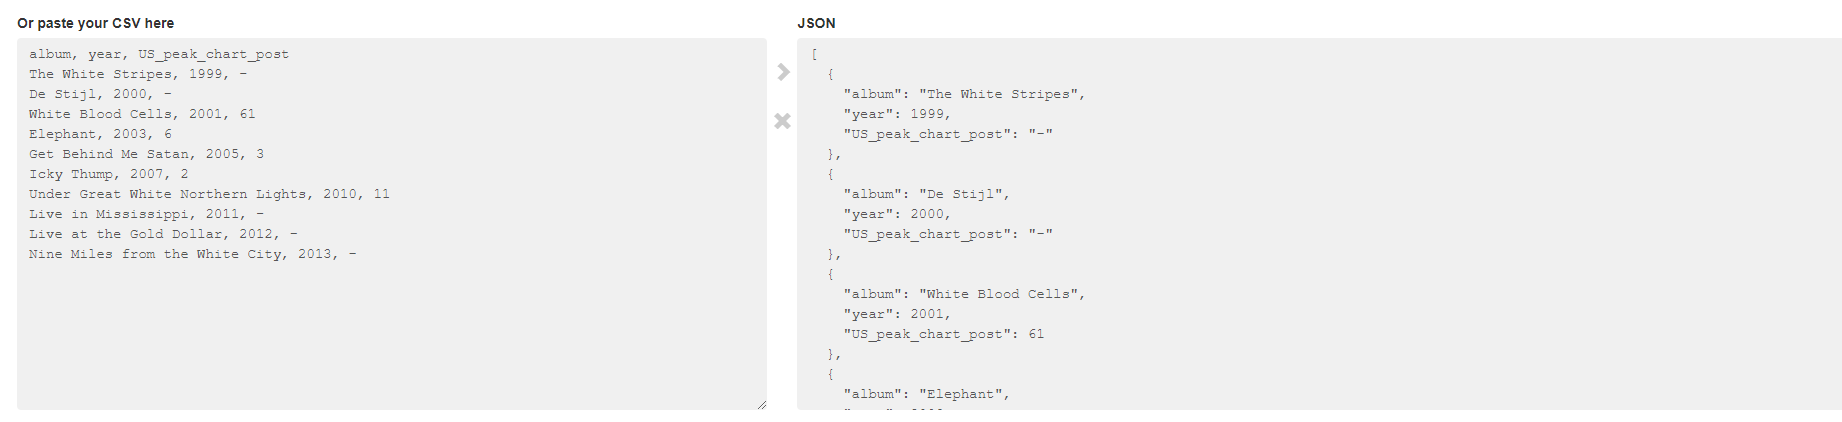
\includegraphics[scale=0.3]{Gambar/json-parser-example}
    \caption{Contoh JSON parser }
    \label{fig:my_label}
\end{figure}


\subsection{\textit{Security Considerations}}
pada umumnya setiap \textit{scripting languages} memiliki masalah keamanan.JSON merupakan bagian dari \textit{javascript} sebaiknya setiap akan melakukan pertuakaran data menggunakan JSON harus melakukan validasi terlebih dahulu agar dapat memastikan kredebilitas dari data yang diterima maupun dikirim.

\section{CSV}
\label{subsec:csv}
CSV (\textit{Comma Separated Values}) adalah suatu format data dalam basis data di mana setiap nilai \textit{atribute} dipisahkan dengan tanda koma (,) dan setiap baris data ditandai dengan baris baru.\cite{RFC:4180} CSV digunakan untuk bertukar data dan mengonversi data dari sebuah program \textit{spreadsheet} ke program \textit{spreadsheet} lainnya. Contoh CSV dapat dilihat pada Listing~\ref{listing:CSV}.

\begin{lstlisting}[caption=Contoh CSV, label=listing:CSV]
    logId,APIKey,Timestamp (UTC),Action,AdditionalData
    113909,E5D9904F0A8B4F99,2/1/2014 0:07,PAGELOAD,/5.10.83.30/
    113910,E5D9904F0A8B4F99,2/1/2014 0:07,PAGELOAD,/5.10.83.49/
\end{lstlisting}


\subsection{\textit{ CSV Grammar}}
\textit{CSV} dapat dituliskan dalam banyak format penulisan. belum ada aturan resmi tentang bagaimana cara penulisan format \textit{CSV}. beberapa aturan dalam penulisan \textit{CSV} yang paling banyak dilakukan adalah:

\begin{itemize}
    \item setiap \textit{record} dipisahkan perbaris , dan dibatasi oleh \textit{line break / (CLRF)} contoh:
            \begin{lstlisting}[]
                 aaa,bbb,ccc CRLF
                 zzz,yyy,xxx CRLF
             \end{lstlisting}
    \item  \textit{record} pada baris terakhir,tidak memerlukan \textit{line break /(CLRF)} contoh:
            \begin{lstlisting}[]
                 aaa,bbb,ccc CRLF
                 zzz,yyy,xxx
             \end{lstlisting}
    \item  dapat menambahkan \textit{header}, header dapat diletakan pada baris pertama \textit{csv} contoh:
            \begin{lstlisting}[]
                 field_name,field_name,field_name CRLF
                 aaa,bbb,ccc CRLF
                 zzz,yyy,xxx
             \end{lstlisting}
    \item  setiap \textit{record} harus memiliki jumlah nilai yang sama, spasi meruapakan bagian dari nilai dan tidak boleh di abaikan contoh:
            \begin{lstlisting}[]
                 aaa,bbb,ccc CRLF
                 zzz,  yyy  ,xxx
             \end{lstlisting}
    \item  penggunaan \textit{double quote ("")} tidak dilarang namun jika ada record yang menggunakan \textit{double quote} sebaiknya harus diimplementasikan untuk seluruh record  contoh:
            \begin{lstlisting}[]
                "aaa","bbb","ccc" CRLF
                 "zzz","yyy","xxx"
             \end{lstlisting}
\end{itemize}

\subsection{\textit{CSV mime type}}
menurut \textit{Internet Assigned Numbers Authority (IANA) CSV } memiliki mime type:
\begin{itemize}
    \item \textit{ MIME media type name: text}
    \item \textit{  MIME subtype name: csv}
    \item \textit{ Required parameters: none}
    \uten \textit{Optional parameters: \textit{charset},\textit{header}}
\end{itemize}

\subsection{\textit{Security considerations}}
\textit{CSV} hanya akan berisi \textit{text} sehingga tidak ada potensi untuk mengakibatkan kerugian. Namun secara \textit{theoretical} memungkinkan untuk meletakan \textit{malicious binary data } untuk melakukan \textit{exploit}.


\section{\textit{Nodejs}}
\textit{Nodejs} adalah  \textit{JavaScript runtime environment } dimana dengan menggunakan \textit{nodejs} memungkinkan untuk menjalankan perintah \textit{ JavaScript} tanpa harus menggunakan \textit{web browser}.\textit{Node JS} memungkinkan \textit{developer} untuk melakukan \textit{server-side scripting} dan menghasilkan \textit{dynamic website}. \cite{Nodejs:01:about}


\subsection{\textit{package management }}
\textit{Package manager} atau \textit{package-management system}  aplikasi yang mengautomatisasi proses \textit{installing}, \textit{upgrade}, dan \textit{delete} suatu aplikasi.\cite{PackageManager:01:about} \textit{NodeJs} dilengkapi dengan sistem \textit{package management} yang bernama \textit{Node Package Module / NPM} yang berguna untuk mengatur dan mengelola \textit{thrid party aplication}.\cite{Nodejs:02:npm}

\subsection{\textit{Architecture}}
\textit{Nodejs} merupakan \textit{event-driven programming} yang memungkinkan \textit{developer} membuat \textit{web server} yang \textit{scalable} tanpa harus menggunakan sistem \textit{threading}.\textit{Nodejs} akan menggunakan \textit{callbacks} sebagai penanda sebuah \textit{event} telah selesai dikerjakan.\textit{Nodejs} dibuat diatas \textit{Google V8 JavaScript engine} dan memiliki lisensi \textit{BSD license}. untuk lisensi \textit{open source}\cite{nodejs:02:platform-arch}.


\section{\textit{Expressjs}}
\textit{Expressjs} adalah \textit{backend framework} untuk \textit{nodejs}. \textit{ExpressJs} dibuat oleh  TJ Holowaychuk.\textit{Expressjs} yang menyediakan \textit{web application} yang \textit{minimalistic} dan \textit{robust}.\cite{Express:01:Mozilla}

\subsection{\textit{Routing}}
\textit{Routing} adalah proses untuk menentukan \textit{path} sehingga aplikasi dapat menentukan perintah yang akan dijalankan berdasarkan path yang sudah ditentukan.\cite{RFC:1332} Pada \textit{expressjs} untuk membuat \textit{routing} \textit{developer} perlu menentukan tiga hal\cite{Express:01:routing}:

\begin{itemize}
    \item \textit{ http Method} yang akan digunakan seperti (\textit{post,get,put}).
    \item \textit{path} yang akan digunakan sebagai alamat route.
    \item \textit{parmeters} nilai yang akan diberikan.
    \item \textit{callback} fungsi yang akan dipanggil begitu proses path route dijalankan. 
\end{itemize}
contoh \textit{syntax routing} pada \textit{expressjs}:
\begin{lstlisting}[]
            // GET method route
                    app.get('/', function (req, res) {
                      res.send('GET request to the homepage')
                    })
                    
                    // POST method route
                    app.post('/', function (req, res) {
                      res.send('POST request to the homepage')
                    })
\end{lstlisting} 

\subsection{\textit{Security Considerations}}
\textit{ExpressJs} telah mendukung fitur \textit{middleware} \cite{Express:01:Security} sehingga \textit{developer} dapat melakukan authentikasi untuk setiap route yang ingin dijalankan.\textit{Middleware} adalah fungsi yang akan dieksekusi sebelum fungsi utama dijalankan.Contoh \textit{syntax middleware}:
\begin{lstlisting}[]
            const myMiddleware = function (req, res, next) {
              console.log('LOGGED')
              next()
            }
            
            app.use(myMiddleware)
            
            app.get('/', function (req, res) {
              res.send('Hello World!')
            })

\end{lstlisting}
Dengan mengimplentasi \textit{code } diatas maka setiap kali \textit{app} menerima even akan mengeluarkan tulisan "LOGGED" pada terminal.



\subsection{\textit{Express file structure }}
Tidak ada aturan resmi untuk menentukan file structure dalam \textit{expressjs}. Namun ada tiga jenis \textit{file structure} yang paling sering digunakan yakni\cite{express:02:FileStructure}:
\begin{itemize}
    \item \textit{Route Listing} dengan menuliskan seluruh \textit{route} pada kelas utama. Contoh:
    \begin{lstlisting}[]
            app.get('/', site.index);
            
            // User
            
            app.get('/users', user.list);
            app.all('/user/:id/:op?', user.load);
            app.get('/user/:id', user.view);
            app.get('/user/:id/view', user.view);
            app.get('/user/:id/edit', user.edit);
            app.put('/user/:id/edit', user.update);
            
            // Posts
            
            app.get('/posts', post.list);
\end{lstlisting}
\item \textit{Route Map} dengan memanfaatkan fungsi \textit{Map} yang disediakan oleh \textit{expressjs}. Contoh: 
    \begin{lstlisting}[]
        app.map({
          '/users': {
            get: users.list,
            delete: users.delete,
            '/:uid': {
              get: users.get,
              '/pets': {
                get: pets.list,
                '/:pid': {
                  delete: pets.delete
                }
              }
            }
          }
        });
\end{lstlisting}

\item \textit{MVC}  memisahkan module \textit{routing} pada \textit{expressjs} menjadi \textit{Model , View ,Controller} 


\end{itemize}

	
\section{Google Maps Javascript API}
\label{sec:googlemaps}
Google Maps adalah layanan pemetaan web yang dikembangkan oleh Google. Menawarkan citra satelit, foto udara, dan peta jalan yang interaktif, kondisi lalu lintas secara \textit{real time} \cite{mehta:19:gmaps}.
 \begin{figure}[H]
    \centering
    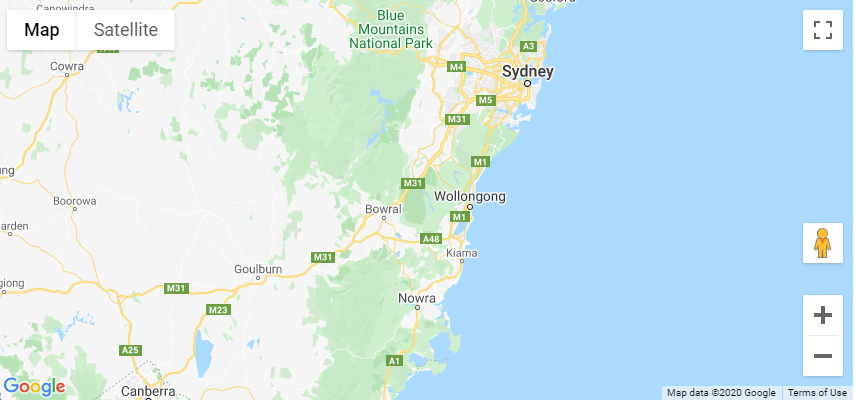
\includegraphics[scale=0.5]{Gambar/example_google_map.PNG}
    \caption{Contoh Heat Map }
    \label{fig:my_label}
\end{figure}
Google Maps dalam service nya telah menyediakan \textit{API (pplication programming interface)} yang dapat di gunakan untuk public.
aplication programming interface adalah \textit{computer interface} yang mengatur komunikasi antar perangkat lunak \cite{libby:20:api}.
Google Maps telah menyediakan beberapa teknik pemetaan data yaitu :
 \begin{itemize}
     \item \textit{Heat Map}
     \item \textit{Marker Clustering}

 \end{itemize}
 terdapat beberapa parmeter untuk menginisialisasi \textit{Google Maps Javascript API}
 \begin{itemize}
     \item \textit{Google Maps Object}
     \item \textit{Position}
     \item \textit{Zoom Level}
 \end{itemize}
 
 \subsection{\textit{Position}}
 \textit{Google Maps} menggunakan \textit{Latitude} dan \textit{Longitude}  sebagai  \textit{atribute} untuk menyatakan sebuah posisi.\cite{GoogleMaps:02:coordinates}
 \textit{Latitude} adalah garis yang horisontal / mendatar. Titik 0 adalah sudut ekuator, tanda + menunjukan arah ke atas menuju kutub utara, sedangkan tanda minus di koordinat Latitude menuju ke kutub selatan. \textit{Longitude} adalah garis lintang . Angka dari sudut bundar bumi horisontal. Titik diawali dari 0 ke 180 derajat, dan 0 ke-180 ke arah sebaliknya.
 \begin{figure}[H]
    \centering
    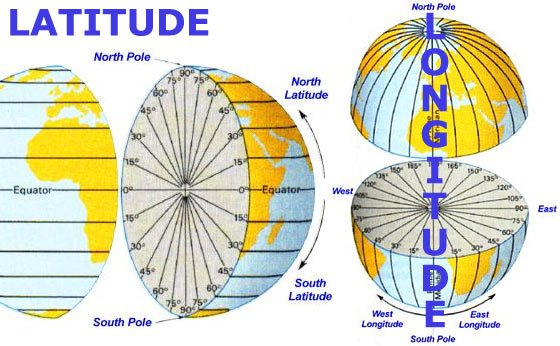
\includegraphics[scale=0.5]{Gambar/definition-of-latitude-longitude.jpg}
    \caption{Contoh Latitude dan Longtitude }
    \label{fig:my_label}
\end{figure}
 
 
 
 \subsection{\textit{Google Maps Object}}
 \textit{Maps Object} adalah Kelas \textit{JavaScript} yang mewakili peta adalah kelas Peta. Objek kelas ini mendefinisikan satu peta di halaman\cite{GoogleMaps:01:MapsObject}. (Anda dapat membuat lebih dari satu \textit{instance} kelas ini - setiap objek akan menentukan peta terpisah pada halaman.) Kami membuat \textit{instance} baru dari kelas ini menggunakan \textit{operator} baru \textit{JavaScript}.
  \begin{lstlisting}
    map = new google.maps.Map(document.getElementById("map"), {...});
 \end{lstlisting}
 \subsection{\textit{Heat Map}}
 \label{subsec:heat map}
 \textit{Heat Map} adalah sebuah teknik visualisasi data dimana data digambarkan sebagai warna. Saat Lapisan \textit{heat map} diaktifkan, hamparan berwarna akan muncul di atas map. Secara  \textit{default}, area dengan intensitas lebih tinggi akan diwarnai merah, dan area dengan intensitas lebih rendah akan tampak hijau.\cite{GoogleMaps:03:heatmap}

 \begin{figure}[H]
    \centering
    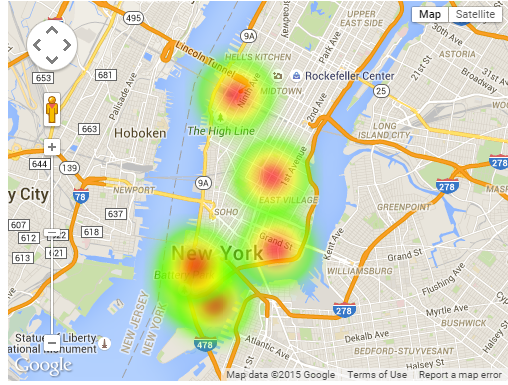
\includegraphics[scale=0.5]{Gambar/heat-map-example}
    \caption{Contoh Heat Map }
    \label{fig:my_label}
\end{figure}

Beberapa Jenis \textit{Heat Map}:
 \begin{itemize}
     \item \textit{Click-tracking map}
     \item \textit{Scroll map}
     \item \textit{Hover/Mouse tracking map}
     \item \textit{Eye tracking map}
 \end{itemize}
 
 Untuk menampilkan \textit{heat map } menggunakan \textit{Google Javascript API} dapat menggunakan syntax.
 \begin{lstlisting}
var heatmap = new google.maps.visualization.HeatmapLayer({
  data: heatMapData
});
heatmap.setMap(map);

\end{lstlisting}
 
 \subsection{\textit{Marker}}
 \label{subsec:heat map}
 \textit{Marker } adalah suatu tanda yang di pasang di dalam sebuah maps atau peta sebagai petanda lokasi atau tempat. Marker  dapat menampilkan gambar khusus, dalam hal ini biasanya disebut sebagai \textit{icon}.\cite{GoogleMarker:01:Maps}.
 Untuk Menambahkan Marker.Untuk menambahkan \textit{Marker} pada \textit{Google Map Javascript Api} membutuhkan beberapa parameter
  \begin{itemize}
     \item \textit{Position}  menggunakan latlng untuk mengidentifikasi letak suatu tempat
     \item \textit{Map} menggunakan object map dari google javascript api
 \end{itemize}
 \begin{figure}[H]
    \centering
    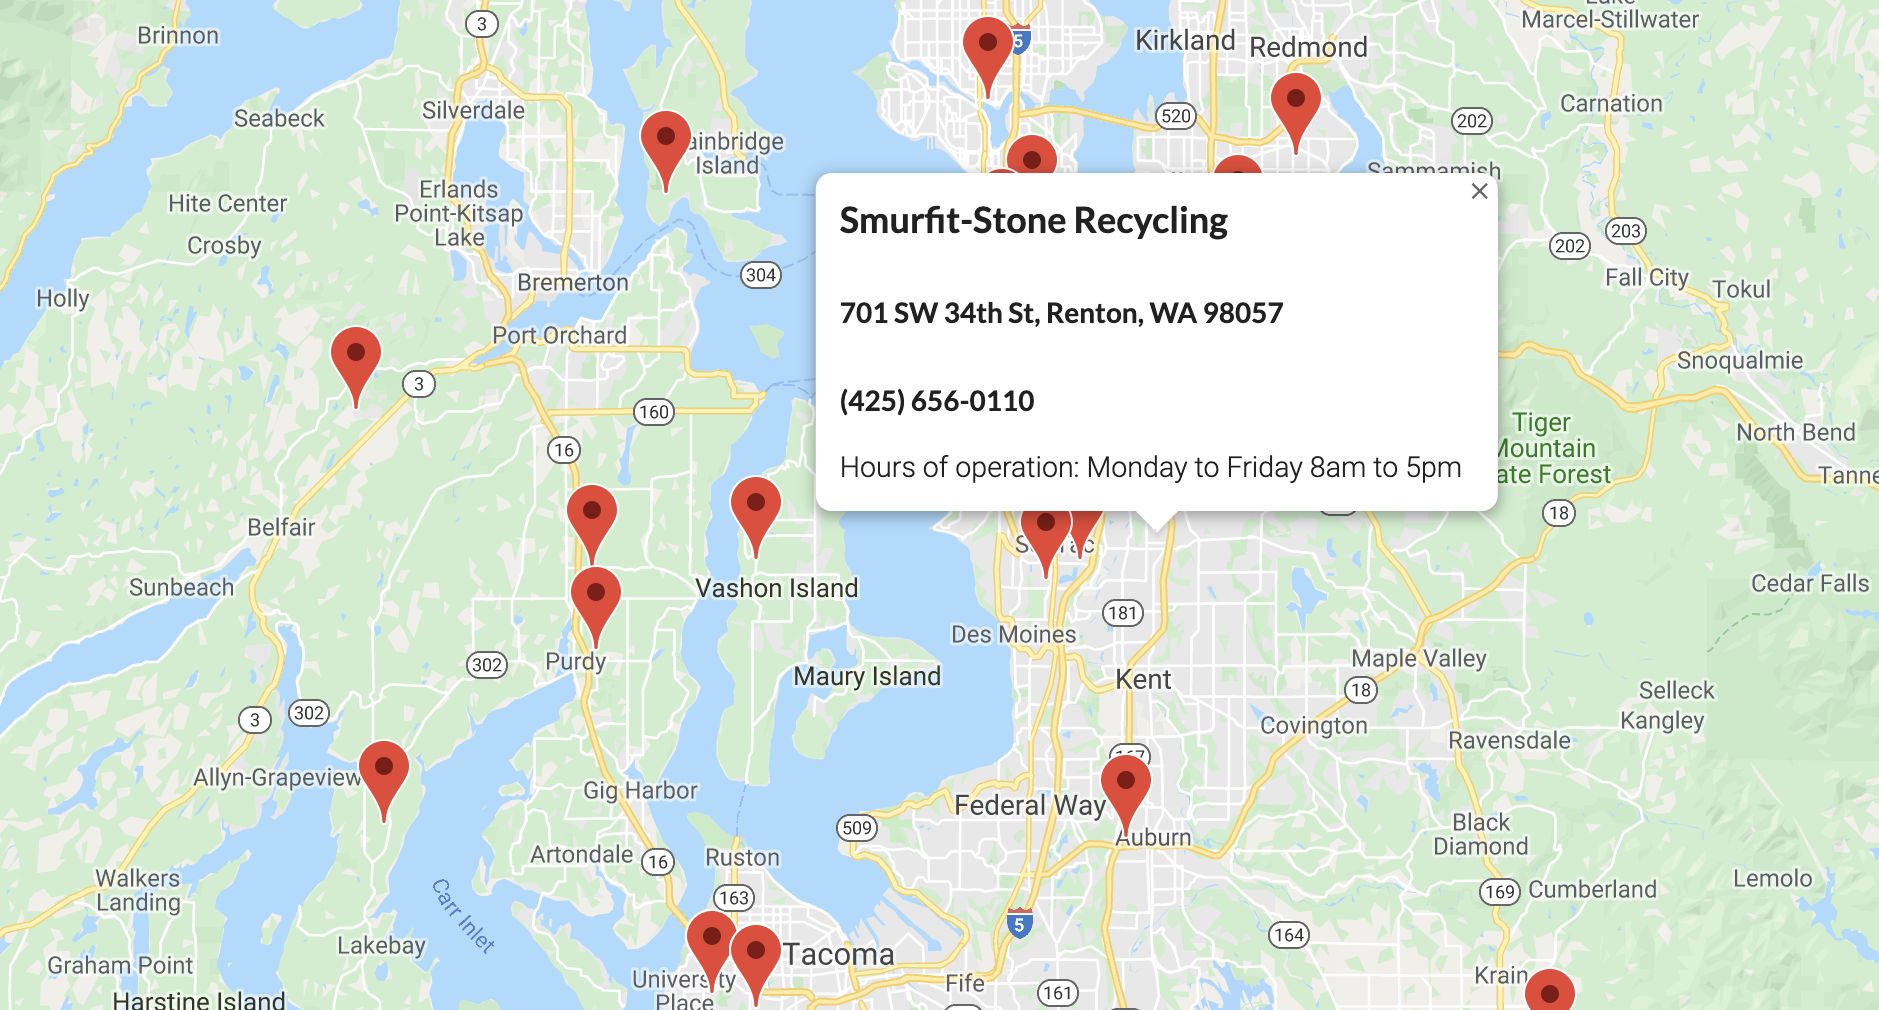
\includegraphics[scale=0.2]{Gambar/marker_example.png}
    \caption{Contoh Marker}
    \label{fig:my_label}
\end{figure}

Untuk menambahkan \textit{Marker} dapat menggunakan \textit{syntax} seperti:
\begin{lstlisting}
var heatmap = new google.maps.visualization.HeatmapLayer({
  data: heatmapData
});
heatmap.setMap(map);

\end{lstlisting}
  \begin{figure}[H]
    \centering
    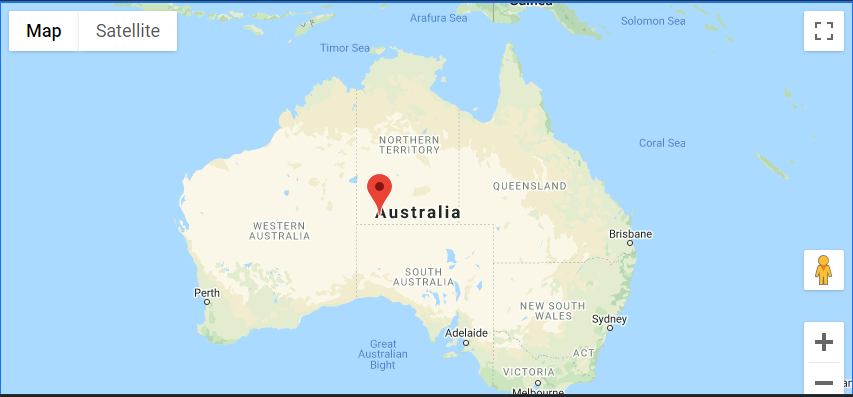
\includegraphics[scale=0.5]{Gambar/add_marker.PNG}
    \caption{Add Marker}
    \label{fig:my_label}
\end{figure}




 
\section{\textit{Marker Clustering}}
 \textit{Marker Clustering } adalah teknik visualisasi data dimana data akan di representasikan sebagai tanda / \textit{Mark} pada suatu space 2 dimensi, semakin banyak data yang terdapat pada suatu tempat maka akan semakin banyak quantitas penanda / \textit{Mark} yang di berikan. \cite{GoogleMarkerCluster:01:Maps}
  \begin{figure}[H]
    \centering
    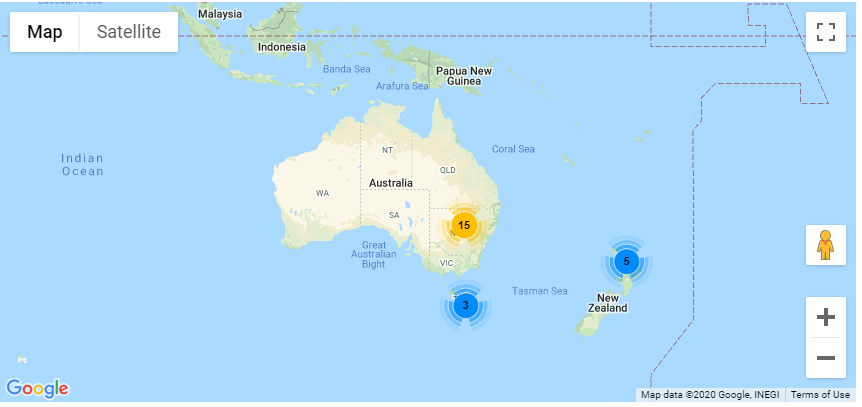
\includegraphics[scale=0.5]{Gambar/marker_clustering.PNG}
    \caption{Contoh Marker Clustering}
    \label{fig:my_label}
\end{figure}
Untuk menggunakan \textit{Marker Clustering} pada \textit{Google Maps Javascript API} dapat menggunakan Object \textit{Marker Clusterer} yang telah di sediakan oleh \textit{Google Maps} 
  \begin{lstlisting}
  new MarkerClusterer(map, markers, {
    imagePath:
      "https://developers.google.com/maps/documentation/javascript/examples/markerclusterer/m",
  });
}
 \end{lstlisting}
 \textit{Marker Clustering} akan menggunakan   \textit{grid-based clustering technique} yang membagi peta menjadi kotak dengan ukuran tertentu (ukuran berubah di setiap tingkat zoom), dan mengelompokkan penanda ke dalam setiap kisi persegi. Ini membuat \textit{cluster} di \textit{marker} tertentu, dan menambahkan marker yang berada dalam batas-batasnya ke \textit{cluster}.\textit{Marker Clustering} merupakan sebuah teknik yang menggunakan \textit{Marker} sehingga untuk dapat memunculkan \textit{Marker Clustering} diperlukan object \textit{Marker}
 berikut ini contoh pengimplenentasian \textit{Marker Clustering}\cite{GoogleMarkerCluster:01:Maps}
 
 \begin{lstlisting}
function initMap() {
  const map = new google.maps.Map(document.getElementById("map"), {
    zoom: 3,
    center: { lat: -28.024, lng: 140.887 },
  });
  const labels = "ABCDEFGHIJKLMNOPQRSTUVWXYZ";
  const markers = locations.map((location, i) => {
    return new google.maps.Marker({
      position: location,
      label: labels[i % labels.length],
    });
  });
  new MarkerClusterer(map, markers, {
    imagePath:"",
  });
}
const locations = [
  { lat: -31.56391, lng: 147.154312 },
  { lat: -33.718234, lng: 150.363181 },
  { lat: -33.727111, lng: 150.371124 },
];
\end{lstlisting}